% !TEX root = ./main.tex

\section{Experimental results}
\label{sec:experiment}

We now present evaluations assessing the viability of our structured prediction approach
for the sequential recommendation task discussed in Section~\ref{sec:trajrec}. 
%of trajectory recommendation.
On two real-world dataset of photo tours, our methods is shown to significantly outperform 
a number of non-structured baselines or those that do not take into account the recommendation setting. 
%, over which we demonstrate significant improvements.


%
\subsection{Photo trajectory datasets}
\label{sec:dataset}

% experiment protocol: Nested cross-validation with Monte-Carlo cross-validation for the inner loop
We assess the recommendation performance %methods developed in Section~\ref{sec:trajrec}
of various methods
on trajectories extracted from Flickr photos
for the cities of Glasgow and Osaka~\cite{thomee2016yfcc100m,ijcai15}.
Each dataset comprises of a
list of trajectories, being a sequence of points of interest (POI), as visited by various Flickr users 
and recorded by the geotags in photos. Photos that are nearby in time and space are grouped and then segmented by eight hours of time gap, visits that only include a single POI are excluded. 
The statistics of datasets are shown in Table~\ref{tab:data}. 
Both datasets are sparse in user activity, 
i.e. each user has on average less than two trajectories. 
This makes user-specific recommendation impractical because of
data availability, and also undesirable because of the domain being urban locations 
-- a user would want different recommendations given different starting locations, and not a static recommendation no matter where she/he is. 
From Table~\ref{tab:data} and Figure~\ref{fig:hist}, 
each distinct query, comprising of start POI and a desired trip length, 
has an average of 4-6, and a maximum of 20-30 trajectories.
Therefore, evaluation is carried out on the problem of recommending trajectories given a query. 
%as posed in \S\ref{sec:trajrec}:
%given a query , can we recommend a trajectory of POIs that a visitor will enjoy?

%A characteristic of these datasets is that many queries are associated with multiple trajectories, or ground truths.
%recommendationThe histograms of the number of ground truths for queries are shown in Figure~\ref{fig:hist}.

% dataset stats
\begin{table}[t]
\caption{Statistics of trajectory dataset}
\label{tab:data}
\centering
\setlength{\tabcolsep}{4pt} % tweak the space between columns
\small
\begin{tabular}{l*{5}{c}} \hline
\textbf{Dataset} & \textbf{\#Traj.} & \textbf{\#POIs} & \textbf{\#Users} & \textbf{\#Queries} & \textbf{AvgLenth} \\ \hline
Osaka            & 186              & 26              & 130              & 47                 & 2.4 \\
Glasgow          & 351              & 25              & 219              & 64                 & 2.5 \\
\hline
\end{tabular}
\end{table}


% histogram of #ground truth
\begin{figure}[t]
	\centering
	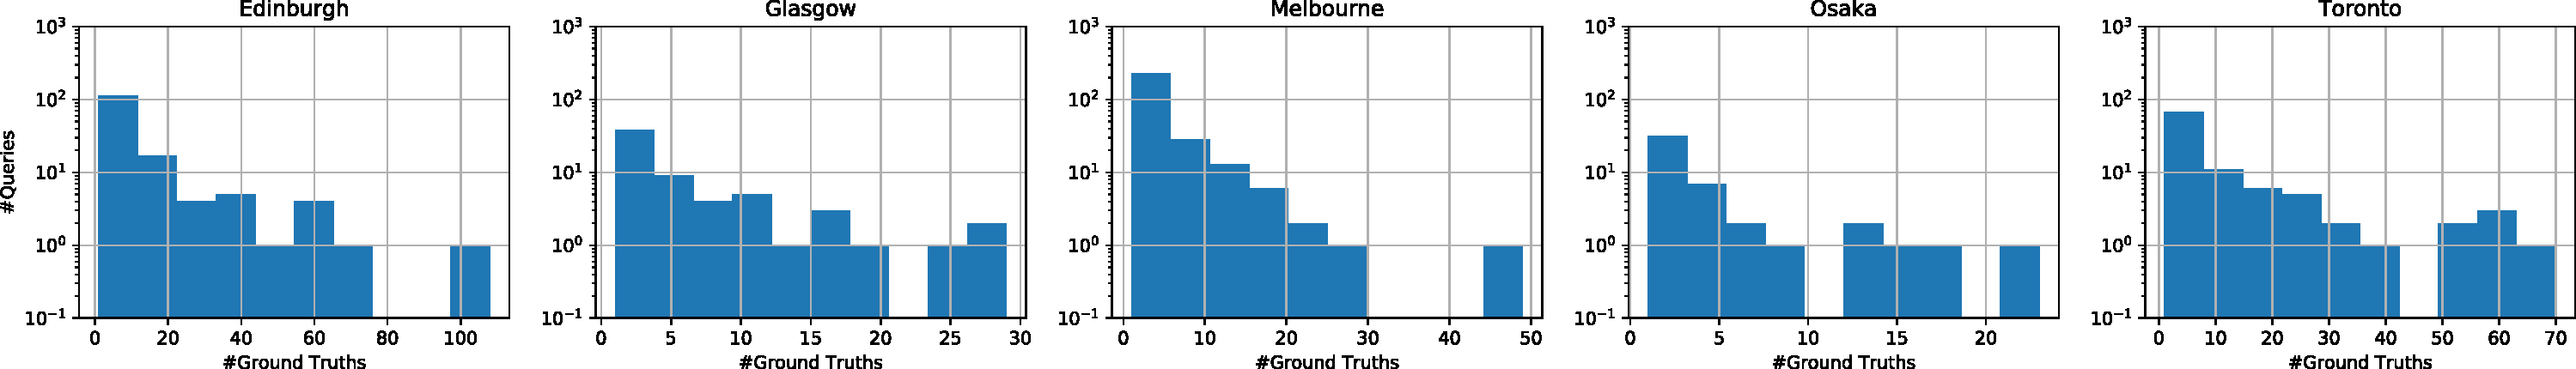
\includegraphics[width=\columnwidth]{hist.pdf}
	\caption{Histograms of the number of trajectories per query.}
	\label{fig:hist}
\end{figure}


%
\subsection{Methods compared}

We compare the performance of our methods to the following three baselines:
\begin{itemize}[leftmargin=0.125in]
\parskip -.05em
	\item The \textsc{Random} baseline simply recommends a sequence of POIs by sampling uniformly at random from the whole set of POIs (without replacement).
	
	\item The stronger \textsc{Popularity} baseline recommends the top-$k$ most popular POIs i.e. the POIs that have been visited the most in the training set.

	\item \textsc{PoiRank}~\cite{cikm16paper} is a generalisation of \textsc{Popularity} which considers a number of POI features in addition to the popularity,
and trains a RankSVM model to learn a score for each POI. The top-$k$ scoring POIs are then used to construct a trajectory.
\end{itemize}

To assess the viability of our structured prediction approach, and the necessity of our two extensions (normalising the loss per query and disallowing loops), we implemented the following versions of our structured prediction methods:
\begin{itemize}[leftmargin=0.125in]
\parskip -.05em
	\item The structured prediction ({\sc SP}) method employs the vanilla structured SVM framework in order to learn a score for trajectories given a query.

	\item The structured recommendation ({\sc SR}) method extends the {\sc SP} method by additionally performing normalisation of the loss function per query,
	so that we do not attempt to distinguish between multiple ground truths for the same query.

	\item The variants {\sc SPpath} and {\sc SRpath} extend the above methods by enforcing the constraint during training that sequences with loops are disallowed.
\end{itemize}


%
\subsection{Evaluation procedure}

% leave-one-out evaluation (with query aggregation)
%As described in Section~\ref{sec:queryagg}, 
To evaluate the performance of the various methods under comparison,
we first group the trajectories according to queries that they conform to.
We then evaluate the performance of each algorithm using leave-one-out cross validation,
where in each iteration of this procedure,
one query and its associated trajectories serves as a test point, with all other trajectories for training.
(Note that without this query aggregation, there will be considerable overlap between the train and test set, and simple nearest neighbour methods will be hard to outperform.)
% model selection (Monte Carlo CV) (with query aggregation): 90/10 random split for 5 times
Furthermore, 
all relevant hyper-parameters (e.g.\ the regularisation constant $C$) are tuned using Monte Carlo cross validation~\cite{burman1989comparative} on the training set.

% evaluation metric: kendall's Tau (mention F1, pF1)
We use three performance measures to assess the test fold performance of each algorithm:
point-F$_1$ score~\cite{ijcai15},
pairs-F$_1$ score~\cite{cikm16paper},
and
Kendall's $\tau$ (version $b$)~\cite{kendall1945,agresti2010analysis}.
\TODO{explain point and pairs}

Kendall's $\tau$
essentially measures the fraction of pairs of POIs that are correctly ordered in the prediction and ground truth sequences,
with adjustment for ties.
In particular,
define the rank of POIs $\mathcal{P}$ in a trajectory $\mathbf{y} = (y_1,\dots,y_K)$ as
the position of the POI within the trajectory,
\begin{align*} 
r_\mathbf{y} &= (r_1,\dots,r_j,\dots,r_{|\mathcal{P}|}), \\
r_j &= \sum_{k=1}^K (| \mathcal{P} | - k + 1)  \llb p_j = y_k \rrb, ~ j = 1, \dots, | \mathcal{P} |.
\end{align*}
The Kendall's $\tau$ score is then computed on $r_\mathbf{y}$ versus $r_\mathbf{\hat{y}}$.
Unlike the F$_1$ scores on points and pairs, 
which only care about the set of correctly recommended POIs or POI pairs,
this metric taking both factors into account.

As described previously, our methods are capable of recommending not merely a single trajectory,
but rather a list of trajectories.
While one can simply take the top recommended trajectory as the prediction,
this ignores the fact that there are likely multiple plausible trajectories for any given query.
Thus, for each performance measure $\mathrm{perf}$,
we take the maximum over all trajectories,
i.e.,
\begin{equation*}
%\tau_b^{(i)} = 
\mathrm{perf}^{(i)}( \mathbf{y}, \hat{\mathbf{y}} ) =
\max_{(\mathbf{y}, \hat{\mathbf{y}}) \in \{\mathbf{y}^{(ij)}\}_{j=1}^{N_i} \times \{\hat{\mathbf{y}}^{(ij)}\}_{j=1}^k} 
%\tau_b(r_\mathbf{y}, r_{\hat{\mathbf{y}}}),
\mathrm{perf}(\mathbf{y}, {\hat{\mathbf{y}}}),
\end{equation*}
where $\{\mathbf{y}^{(ij)}\}_{j=1}^{N_i}$ are the ground truths for query $\mathbf{x}^{(i)}$ and
$\{\hat{\mathbf{y}}^{(ij)}\}_{j=1}^k$ are the top-$k$ recommendations.


\secmoveup
\subsection{Results and discussion}
\label{sec:result}
\textmoveup

% !TEX root = ./main.tex

\begin{table*}[t]
\caption{Experimental results on trajectory recommendation datasets. The top three rows are baselines, and the bottom four are the methods proposed in this paper. Bolded entries correspond to the best performing method for each metric; italicised entries to the next best method. Higher scores are better.}
\label{tab:result}
\centering
%\setlength{\tabcolsep}{3pt} % tweak the space between columns
\small
\begin{tabular}{l|cc|cc|cc} \hline
                    & \multicolumn{2}{|c}{\textbf{Kendall's $\tau$}}
                    & \multicolumn{2}{|c}{\textbf{F$_1$ score on points}}
                    & \multicolumn{2}{|c}{\textbf{F$_1$ score on pairs}} \\ \cline{2-7}
                    & Osaka & Glasgow 
                    & Osaka & Glasgow  
                    & Osaka & Glasgow \\ \hline
\textsc{Random}     & $0.403\pm0.025$ & $0.410\pm0.032$  
                    & $0.430\pm0.021$ & $0.451\pm0.027$  
                    & $0.057\pm0.024$ & $0.136\pm0.037$ \\
\textsc{Popularity} & $0.567\pm0.034$ & $0.646\pm0.035$  
                    & $0.601\pm0.031$ & $0.681\pm0.032$  
                    & $0.277\pm0.051$ & $0.416\pm0.050$ \\
\textsc{PoiRank}    & $0.646\pm0.040$ & $0.736\pm0.030$  
                    & $0.678\pm0.037$ & $0.764\pm0.027$  
                    & $0.425\pm0.058$ & $0.550\pm0.047$ \\
\midrule
\textsc{SP}         & $0.796\pm0.037$ & $0.865\pm0.027$  
                    & $0.817\pm0.034$ & $0.878\pm0.024$  
                    & $0.665\pm0.055$ & $0.772\pm0.040$ \\
\textsc{SPpath}     & $0.794\pm0.035$ & $0.740\pm0.034$  
                    & $0.814\pm0.032$ & $0.764\pm0.030$  
                    & $0.653\pm0.054$ & $0.591\pm0.047$ \\
\textsc{SR}         & $\mathbf{0.814\pm0.034}$ & $\mathit{0.870\pm0.025}$  
                    & $\mathbf{0.832\pm0.031}$ & $\mathit{0.887\pm0.022}$ 
                    & $\mathit{0.673\pm0.053}$ & $\mathit{0.774\pm0.039}$ \\
\textsc{SRpath}     & $\mathit{0.805\pm0.036}$ & $\mathbf{0.877\pm0.025}$ 
                    & $\mathit{0.821\pm0.033}$ & $\mathbf{0.893\pm0.021}$ 
                    & $\mathbf{0.682\pm0.054}$ & $\mathbf{0.792\pm0.038}$ \\ \hline
\end{tabular}
\end{table*}


% experimental results
The performance of three baselines and four variants based on structured prediction on two datasets are shown in Table~\ref{tab:result}.
From these results, we can make the following key inferences that validate our contributions.

\textbf{Exploiting the structure of sequences helps}.
We find that all variants of our structured prediction methods achieve better performance than existing baselines.
This indicates that the basis of our approach -- reducing sequence recommendation to a structured prediction problem -- is sensible, and has empirical benefit.

\textbf{Accounting for multiple ground truths helps}.
We find that \textsc{SR} always performs better than \textsc{SP},
and similarly for the {\sc path} variants of both methods. 
This indicates that our first extension -- explicitly modelling multiple ground truths helps recommendation -- is important to achieve good performance.
(We note that even without this correction, our structured methods outperform baselines.)

\textbf{Eliminating loops during training helps}.
We find that {\sc SRpath} improves performance further of the {\sc SR} method,
as indicated by the F$_1$ score on pairs.
This indicates that our second extension -- explicitly performing sub-tour elimination in training -- is important to further improve performance.
Interestingly,
this advantage does \emph{not} take effect if the multiple ground truths are not modelled explicitly,
with the performance of the {\sc SP} method largely unaffected.

\textbf{An illustrative example}. Figure~\ref{fig:example} consist of an example that illustrates the difference among the different algorithm variants. The query requires the trajectory to start from the middle point and be of length 2. 
\textsc{PoiRank} regards points at the lower right and upper left be of the highest rank, but did not consider their compatibility (\ie pairwise features). {\sc SP} and {\sc SR} hits one edge out of the two the groundtruth (green edge), while {\sc SRpath} hits both edges for two valid trajectories after taking all factors into account. 

Overall, these results indicate that our structured prediction approach to the problem has
benefits over non-structured approaches,
and that our extensions to the vanilla structured approach are important to further improve performance.

%\subsection{Example}
%\label{sec:example}

\begin{figure*}[t]
	\centering
	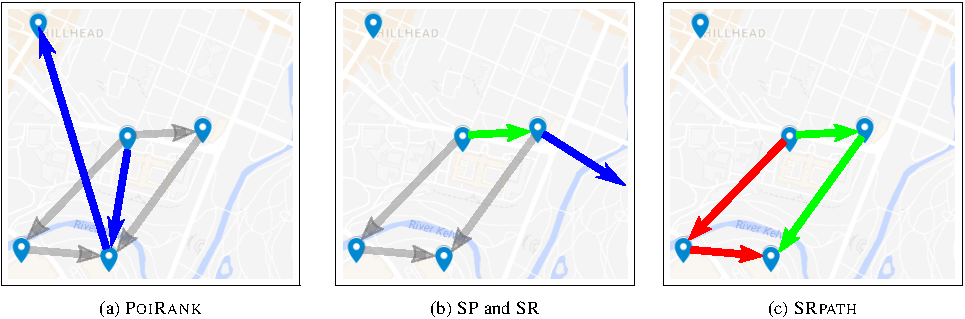
\includegraphics[width=0.99\textwidth]{example.pdf}
	\caption{Example of structured recommender versus baseline on a query with two ground truths as shown in Figure (c). 
             (a) \textsc{PoiRank} cannot make a recommendation related to any of the ground truths; 
             (b) \textsc{SP} and \textsc{SR} recommend a better trajectory than \textsc{PoiRank}, but not fully consistent with the ground truths;
             (c) \textsc{SRpath} hit both ground truths at rank 3 and 5 respectively.}
	\label{fig:example}
\end{figure*}


